\documentclass{sigcomm-alternate}

\begin{document}

\title{Net Neutrality, Bandwidth Usage and Government Regulations}
	
\numberofauthors{3}

\author{
	% 1st. author
	\alignauthor
	Raz Friman\\
	\affaddr{Southern Methodist Univeristy}\\
	\affaddr{5600 SMU Blvd. APT 1516}\\
	\affaddr{Dallas, Texas, 75206}\\
	\email{rfriman@smu.edu}
	% 2nd. author
	\alignauthor
	Jarret Shook\\
	\affaddr{Southern Methodist Univeristy}\\
	\affaddr{5555 Amesbury Dr. APT 1303}\\
	\affaddr{Dallas, Texas, 75206}\\
	\email{jshook@smu.edu}
	% 3rd. author
	\alignauthor Elena Villamil\\
	\affaddr{Southern Methodist Univeristy}\\
	\affaddr{5555 Amesbury Dr. APT 1303}\\
	\affaddr{Dallas, Texas, 75206}\\
	\email{mvillamilrod@smu.edu}
	\and  % use '\and' if you need 'another row' of author names	
	% 4th. author
	\alignauthor Jeffrey Artigues\\
	\affaddr{Southern Mehthodist University}\\
	\affaddr{9520 Amberton Pkwy.}\\
	\affaddr{Dallas, Texas, 75243}\\
	\email{jartigues@smu.edu}
}

\maketitle

\begin{abstract}
Abstract (Problem Statement, Motivation, Conclusion): 
This paper will focus on the impact of laws enforcing Net Neutrality and the regulations of the Internet as a utility. Net Neutrality is a widely debated technical topic that is being discussed politically.  The political discussions broaden the topic to focus on more than just the technical aspects, specifically the impacts net neutrality would have on the economic, political and business environments. In this paper, we will explore how bandwidth usage is affected by Net Neutrality, how prioritization can affect the network, how other countries which have implemented Net Neutrality compare to the US, and the economic implications of Net Neutrality. CONCLUSIONS.

\end{abstract}



\section{Introduction}
Introduction: (Motivation, Problem Statement, Basic Approach, Primary Conclusions, Summary of Outline)

[Motivation] In February 2014, Netflix issued a class action lawsuit against Comcast stating it was illegal for Comcast to throttle back Netflix speeds due to bandwidth usage.  The lawsuit ended with Netflix settling out of court with Comcast. This lawsuit proved that there is current no net neutrality in the United States. This was a big motivation for reviewing regulations on Internet, not just in the US but also in Europe. Additionally, Japan has already implemented regulations in order to preserve Net Neutrality. Furthermore, two of the main foci of the latest bill passed by the FCC are to establish Net Neutrality and to regulate the Internet as utility. [Problem Statement]The question is how do these laws, in particular regulating internet as a utility, politically and economically affect the country, and how they affect the quality of service of Internet. 

[Basic Approach]First, we define Net Neutrality as: “[the] principle according to which all internet traffic is treated equally, whithout discrimination, restriction or interference, independtly of its sender, recipient, type, content, device, service or applciation” [https://gigaom.com/2014/04/03/european-parliament-passes-strong-net-neutrality-law-along-with-major-roaming-reforms/]. First, we analyze current network traffic and draw conclusion on how net neutrality would affect this usage. Network traffic is significantly increasing, and in particular video streaming is the one increasing the most rapidly. As of today this bandwidth usage is not a pro 

[Primary conclusions]

[Summary of Outline] We start with an analyze of the current bandwidth usage. Then we expose an overview of the current bill passed by the FCC. In a later section we will discuss its different political, economical and technical implications while we comparing them to Japan and Europe’s model. Lastly, we will present our conclusions


\section{Related Work}
There is an ever-growing collection of publications, articles, and news reports about Net Neutrality. Unfortunately, almost all of these sources usually include some degree of bias in them. In order to get unbiased information about this topic, we have to analyze multiple sources with all levels of bias from each side and combine their factual information together to get a better understanding of Net Neutrality. This includes reading Whitepapers published by major ISPs in addition to the articles published by the FCC favoring their Net Neutrality proposal. By combining these two heavily baised sources, we can extract the actual relevant information and create a view that is not biased towards any one side.

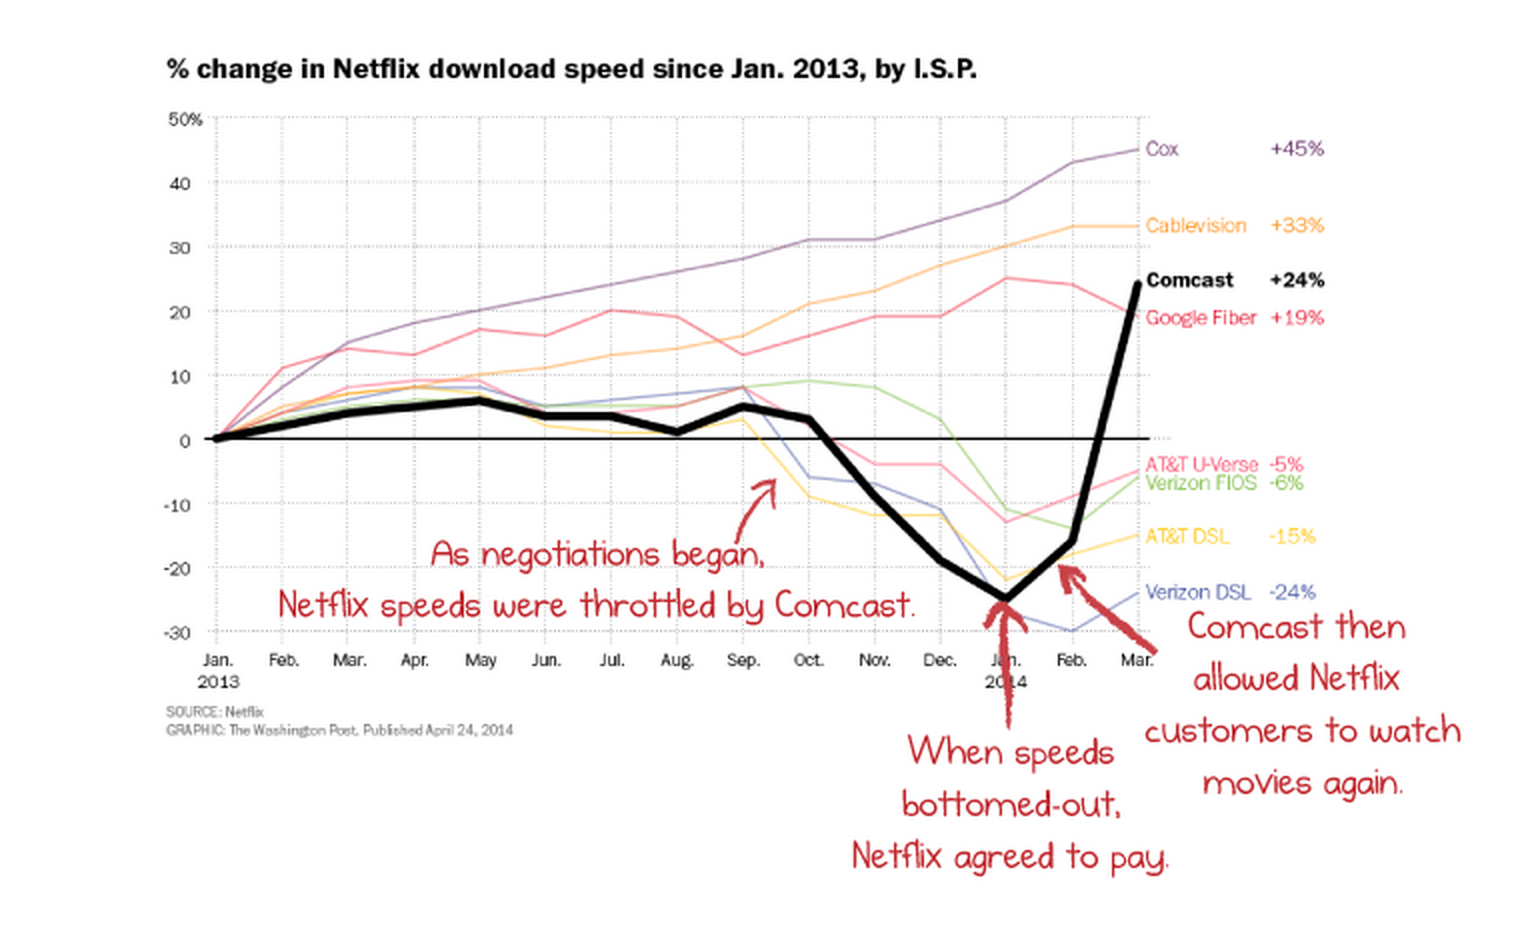
\includegraphics[scale=.15]{NetflixGraph.png}


\section{Research Approach}

\subsection{Bandwidth}
As we transition into an even more interconnected world with the Internet of Things, real time information most likely in small quantities is expected to be in high demand and readily available.


\section{Conclusions}
We have concluded that ISP....



\bibliographystyle{unsrt}
\bibliography{bib}

\end{document}
